% Options for packages loaded elsewhere
% Options for packages loaded elsewhere
\PassOptionsToPackage{unicode}{hyperref}
\PassOptionsToPackage{hyphens}{url}
\PassOptionsToPackage{dvipsnames,svgnames,x11names}{xcolor}
%
\documentclass[
  number]{elsarticle}
\usepackage{xcolor}
\usepackage{amsmath,amssymb}
\setcounter{secnumdepth}{5}
\usepackage{iftex}
\ifPDFTeX
  \usepackage[T1]{fontenc}
  \usepackage[utf8]{inputenc}
  \usepackage{textcomp} % provide euro and other symbols
\else % if luatex or xetex
  \usepackage{unicode-math} % this also loads fontspec
  \defaultfontfeatures{Scale=MatchLowercase}
  \defaultfontfeatures[\rmfamily]{Ligatures=TeX,Scale=1}
\fi
\usepackage{lmodern}
\ifPDFTeX\else
  % xetex/luatex font selection
\fi
% Use upquote if available, for straight quotes in verbatim environments
\IfFileExists{upquote.sty}{\usepackage{upquote}}{}
\IfFileExists{microtype.sty}{% use microtype if available
  \usepackage[]{microtype}
  \UseMicrotypeSet[protrusion]{basicmath} % disable protrusion for tt fonts
}{}
\makeatletter
\@ifundefined{KOMAClassName}{% if non-KOMA class
  \IfFileExists{parskip.sty}{%
    \usepackage{parskip}
  }{% else
    \setlength{\parindent}{0pt}
    \setlength{\parskip}{6pt plus 2pt minus 1pt}}
}{% if KOMA class
  \KOMAoptions{parskip=half}}
\makeatother
% Make \paragraph and \subparagraph free-standing
\makeatletter
\ifx\paragraph\undefined\else
  \let\oldparagraph\paragraph
  \renewcommand{\paragraph}{
    \@ifstar
      \xxxParagraphStar
      \xxxParagraphNoStar
  }
  \newcommand{\xxxParagraphStar}[1]{\oldparagraph*{#1}\mbox{}}
  \newcommand{\xxxParagraphNoStar}[1]{\oldparagraph{#1}\mbox{}}
\fi
\ifx\subparagraph\undefined\else
  \let\oldsubparagraph\subparagraph
  \renewcommand{\subparagraph}{
    \@ifstar
      \xxxSubParagraphStar
      \xxxSubParagraphNoStar
  }
  \newcommand{\xxxSubParagraphStar}[1]{\oldsubparagraph*{#1}\mbox{}}
  \newcommand{\xxxSubParagraphNoStar}[1]{\oldsubparagraph{#1}\mbox{}}
\fi
\makeatother


\usepackage{longtable,booktabs,array}
\usepackage{calc} % for calculating minipage widths
% Correct order of tables after \paragraph or \subparagraph
\usepackage{etoolbox}
\makeatletter
\patchcmd\longtable{\par}{\if@noskipsec\mbox{}\fi\par}{}{}
\makeatother
% Allow footnotes in longtable head/foot
\IfFileExists{footnotehyper.sty}{\usepackage{footnotehyper}}{\usepackage{footnote}}
\makesavenoteenv{longtable}
\usepackage{graphicx}
\makeatletter
\newsavebox\pandoc@box
\newcommand*\pandocbounded[1]{% scales image to fit in text height/width
  \sbox\pandoc@box{#1}%
  \Gscale@div\@tempa{\textheight}{\dimexpr\ht\pandoc@box+\dp\pandoc@box\relax}%
  \Gscale@div\@tempb{\linewidth}{\wd\pandoc@box}%
  \ifdim\@tempb\p@<\@tempa\p@\let\@tempa\@tempb\fi% select the smaller of both
  \ifdim\@tempa\p@<\p@\scalebox{\@tempa}{\usebox\pandoc@box}%
  \else\usebox{\pandoc@box}%
  \fi%
}
% Set default figure placement to htbp
\def\fps@figure{htbp}
\makeatother





\setlength{\emergencystretch}{3em} % prevent overfull lines

\providecommand{\tightlist}{%
  \setlength{\itemsep}{0pt}\setlength{\parskip}{0pt}}



 
\usepackage[]{natbib}
\bibliographystyle{plainnat}


\makeatletter
\@ifpackageloaded{float}{}{\usepackage{float}}
\floatstyle{plain}
\@ifundefined{c@chapter}{\newfloat{suppfig}{h}{lofigs}}{\newfloat{suppfig}{h}{lofigs}[chapter]}
\floatname{suppfig}{Figure S}
\newcommand*\quartofigsref[1]{Fig \hyperref[#1]{S\ref{#1}}}
\@ifpackageloaded{caption}{}{\usepackage{caption}}
\DeclareCaptionLabelFormat{quartofigsreflabelformat}{#1#2}
\captionsetup[suppfig]{labelformat=quartofigsreflabelformat}
\newcommand*\listofsuppfigs{\listof{suppfig}{List of Fig Ss}}
\makeatother
\makeatletter
\@ifpackageloaded{float}{}{\usepackage{float}}
\floatstyle{plain}
\@ifundefined{c@chapter}{\newfloat{supptab}{h}{lotbls}}{\newfloat{supptab}{h}{lotbls}[chapter]}
\floatname{supptab}{Table S}
\newcommand*\quartotblsref[1]{Table \hyperref[#1]{S\ref{#1}}}
\@ifpackageloaded{caption}{}{\usepackage{caption}}
\DeclareCaptionLabelFormat{quartotblsreflabelformat}{#1#2}
\captionsetup[supptab]{labelformat=quartotblsreflabelformat}
\newcommand*\listofsupptabs{\listof{supptab}{List of Table Ss}}
\makeatother
\makeatletter
\@ifpackageloaded{caption}{}{\usepackage{caption}}
\AtBeginDocument{%
\ifdefined\contentsname
  \renewcommand*\contentsname{Table of contents}
\else
  \newcommand\contentsname{Table of contents}
\fi
\ifdefined\listfigurename
  \renewcommand*\listfigurename{List of Figures}
\else
  \newcommand\listfigurename{List of Figures}
\fi
\ifdefined\listtablename
  \renewcommand*\listtablename{List of Tables}
\else
  \newcommand\listtablename{List of Tables}
\fi
\ifdefined\figurename
  \renewcommand*\figurename{Figure}
\else
  \newcommand\figurename{Figure}
\fi
\ifdefined\tablename
  \renewcommand*\tablename{Table}
\else
  \newcommand\tablename{Table}
\fi
}
\@ifpackageloaded{float}{}{\usepackage{float}}
\floatstyle{ruled}
\@ifundefined{c@chapter}{\newfloat{codelisting}{h}{lop}}{\newfloat{codelisting}{h}{lop}[chapter]}
\floatname{codelisting}{Listing}
\newcommand*\listoflistings{\listof{codelisting}{List of Listings}}
\makeatother
\makeatletter
\usepackage{pdflscape}
\makeatother
\makeatletter
\makeatother
\makeatletter
\@ifpackageloaded{caption}{}{\usepackage{caption}}
\@ifpackageloaded{subcaption}{}{\usepackage{subcaption}}
\makeatother
\journal{International Journal of Antimicrobial Agents}
\usepackage{bookmark}
\IfFileExists{xurl.sty}{\usepackage{xurl}}{} % add URL line breaks if available
\urlstyle{same}
\hypersetup{
  pdftitle={A fluconazole population pharmacokinetics study to improve target attainment in critically ill patients},
  pdfauthor={My-Luong Vuong; Omar Elkayal; Ruth Van Daele; Jan-Willem C. Alffenaar; Sophie L. Stocker; Jason A. Roberts; Yves Debaveye; Joost Wauters; Beatrijs Mertens; Jasper M. Boonstra; Indy Sandaradura; Deborah J.E. Marriott; Roger J. Brüggemann; Jeroen A. Schouten; Raoul Bergner; Steven Buijk; Isabel Spriet; Erwin Dreesen},
  colorlinks=true,
  linkcolor={blue},
  filecolor={Maroon},
  citecolor={Blue},
  urlcolor={Blue},
  pdfcreator={LaTeX via pandoc}}


\setlength{\parindent}{6pt}
\begin{document}

\begin{frontmatter}
\title{A fluconazole population pharmacokinetics study to improve target
attainment in critically ill patients}
\author[1]{My-Luong Vuong%
%
}
 \ead{myluong.vuong@kuleuven.be} 
\author[1]{Omar Elkayal%
%
}
 \ead{omarelkayal@hotmail.com} 
\author[1,2]{Ruth Van Daele%
%
}

\author[3,4,5]{Jan-Willem C. Alffenaar%
%
}

\author[3,5,6,7]{Sophie L. Stocker%
%
}

\author[8,9,10]{Jason A. Roberts%
%
}

\author[11,12]{Yves Debaveye%
%
}

\author[13,12]{Joost Wauters%
%
}

\author[1,2]{Beatrijs Mertens%
%
}

\author[14]{Jasper M. Boonstra%
%
}

\author[15,16,17]{Indy Sandaradura%
%
}

\author[18,19]{Deborah J.E. Marriott%
%
}

\author[20,21]{Roger J. Brüggemann%
%
}

\author[22]{Jeroen A. Schouten%
%
}

\author[23]{Raoul Bergner%
%
}

\author[24]{Steven Buijk%
%
}

\author[2]{Isabel Spriet%
%
}
 \ead{isabel.spriet@uzleuven.be} 
\author[1]{Erwin Dreesen%
\corref{cor1}%
}
 \ead{erwin.dreesen@kuleuven.be} 

\affiliation[1]{organization={KU Leuven, Department of Pharmaceutical
and Pharmacological
Sciences},city={Leuven},country={Belgium},countrysep={,},postcodesep={}}
\affiliation[2]{organization={University Hospitals Leuven, Pharmacy
Department},city={Leuven},country={Belgium},countrysep={,},postcodesep={}}
\affiliation[3]{organization={The University of Sydney, School of
Pharmacy, Faculty of Medicine and
Health},city={Sydney},country={Australia},countrysep={,},postcodesep={}}
\affiliation[4]{organization={Westmead Hospital, Pharmacy
Department},city={Sydney},country={Australia},countrysep={,},postcodesep={}}
\affiliation[5]{organization={The University of Sydney, Institute for
Infectious Diseases (Sydney
ID)},city={Sydney},country={Australia},countrysep={,},postcodesep={}}
\affiliation[6]{organization={University of New South Wales, School of
Clinical Medicine, Faculty of Medicine and
Health},city={Sydney},country={Australia},countrysep={,},postcodesep={}}
\affiliation[7]{organization={St.~Vincent's Hospital, Department of
Clinical Pharmacology and
Toxicology},city={Sydney},country={Australia},countrysep={,},postcodesep={}}
\affiliation[8]{organization={The University of Queensland, University
of Queensland Centre for Clinical Research
(UQCCR)},city={Brisbane},country={Australia},countrysep={,},postcodesep={}}
\affiliation[9]{organization={Royal Brisbane and Women's
Hospital, Departments of Pharmacy and Intensive Care
Medicine},city={Brisbane},country={Australia},countrysep={,},postcodesep={}}
\affiliation[10]{organization={University of Montpellier, Division of
Anaesthesiology Critical Care Emergency and Pain Medicine, Nîmes
University
Hospital},city={Nîmes},country={France},countrysep={,},postcodesep={}}
\affiliation[11]{organization={KU Leuven, Department of Cellular and
Molecular
Medicine},city={Leuven},country={Belgium},countrysep={,},postcodesep={}}
\affiliation[12]{organization={University Hospitals Leuven, Medical
Intensive Care
Unit},city={Leuven},country={Belgium},countrysep={,},postcodesep={}}
\affiliation[13]{organization={KU Leuven, Department of Microbiology,
Immunology and
Transplantation},city={Leuven},country={Belgium},countrysep={,},postcodesep={}}
\affiliation[14]{organization={University of Groningen, Department of
Clinical Pharmacy and Pharmacology, University Medical Centre
Groningen},city={Groningen},country={The
Netherlands},countrysep={,},postcodesep={}}
\affiliation[15]{organization={Westmead Hospital, Centre for Infectious
Diseases and
Microbiology},city={Sydney},country={Australia},countrysep={,},postcodesep={}}
\affiliation[16]{organization={The University of Sydney, Faculty of
Medicine and Health, Westmead Clinical
School},city={Sydney},country={Australia},countrysep={,},postcodesep={}}
\affiliation[17]{organization={Westmead Hospital, Institute of Clinical
Pathology and Medical Research, New South Wales Health
Pathology},city={Sydney},country={Australia},countrysep={,},postcodesep={}}
\affiliation[18]{organization={UNSW Sydney, School of Clinical Medicine,
St Vincent's Healthcare Clinical Campus, Faculty of Medicine and
Health},city={Sydney},country={Australia},countrysep={,},postcodesep={}}
\affiliation[19]{organization={St.~Vincent's Hospital, Clinical
Microbiology and Infectious Diseases
Department},city={Sydney},country={Australia},countrysep={,},postcodesep={}}
\affiliation[20]{organization={Radboud university medical
centre, Radboud Institute for Medical Innovations, Department of
Pharmacy},city={Nijmegen},country={The
Netherlands},countrysep={,},postcodesep={}}
\affiliation[21]{organization={Radboud university medical center/CWZ
hospital, Centre of Expertise in Mycology},city={Nijmegen},country={The
Netherlands},countrysep={,},postcodesep={}}
\affiliation[22]{organization={Canisius Wilhelmina Hospital, Department
of Intensive Care},city={Nijmegen},country={The
Netherlands},countrysep={,},postcodesep={}}
\affiliation[23]{organization={Ludwigshafen Medical Centre, Division of
Rheumatology and Nephrology, Department of Medicine
A},city={Ludwigshafen},country={Germany},countrysep={,},postcodesep={}}
\affiliation[24]{organization={Department of Surgery, IJsseland
Hospital},city={Capelle aan den
Ijssel},country={Germany},countrysep={,},postcodesep={}}

\cortext[cor1]{Corresponding author}


















        





\end{frontmatter}
    

\begin{landscape}

\section*{Supplementary Figures}
\addcontentsline{toc}{section}{Supplementary Figures}
\phantomsection

\vspace{1em}
\begin{suppfig}

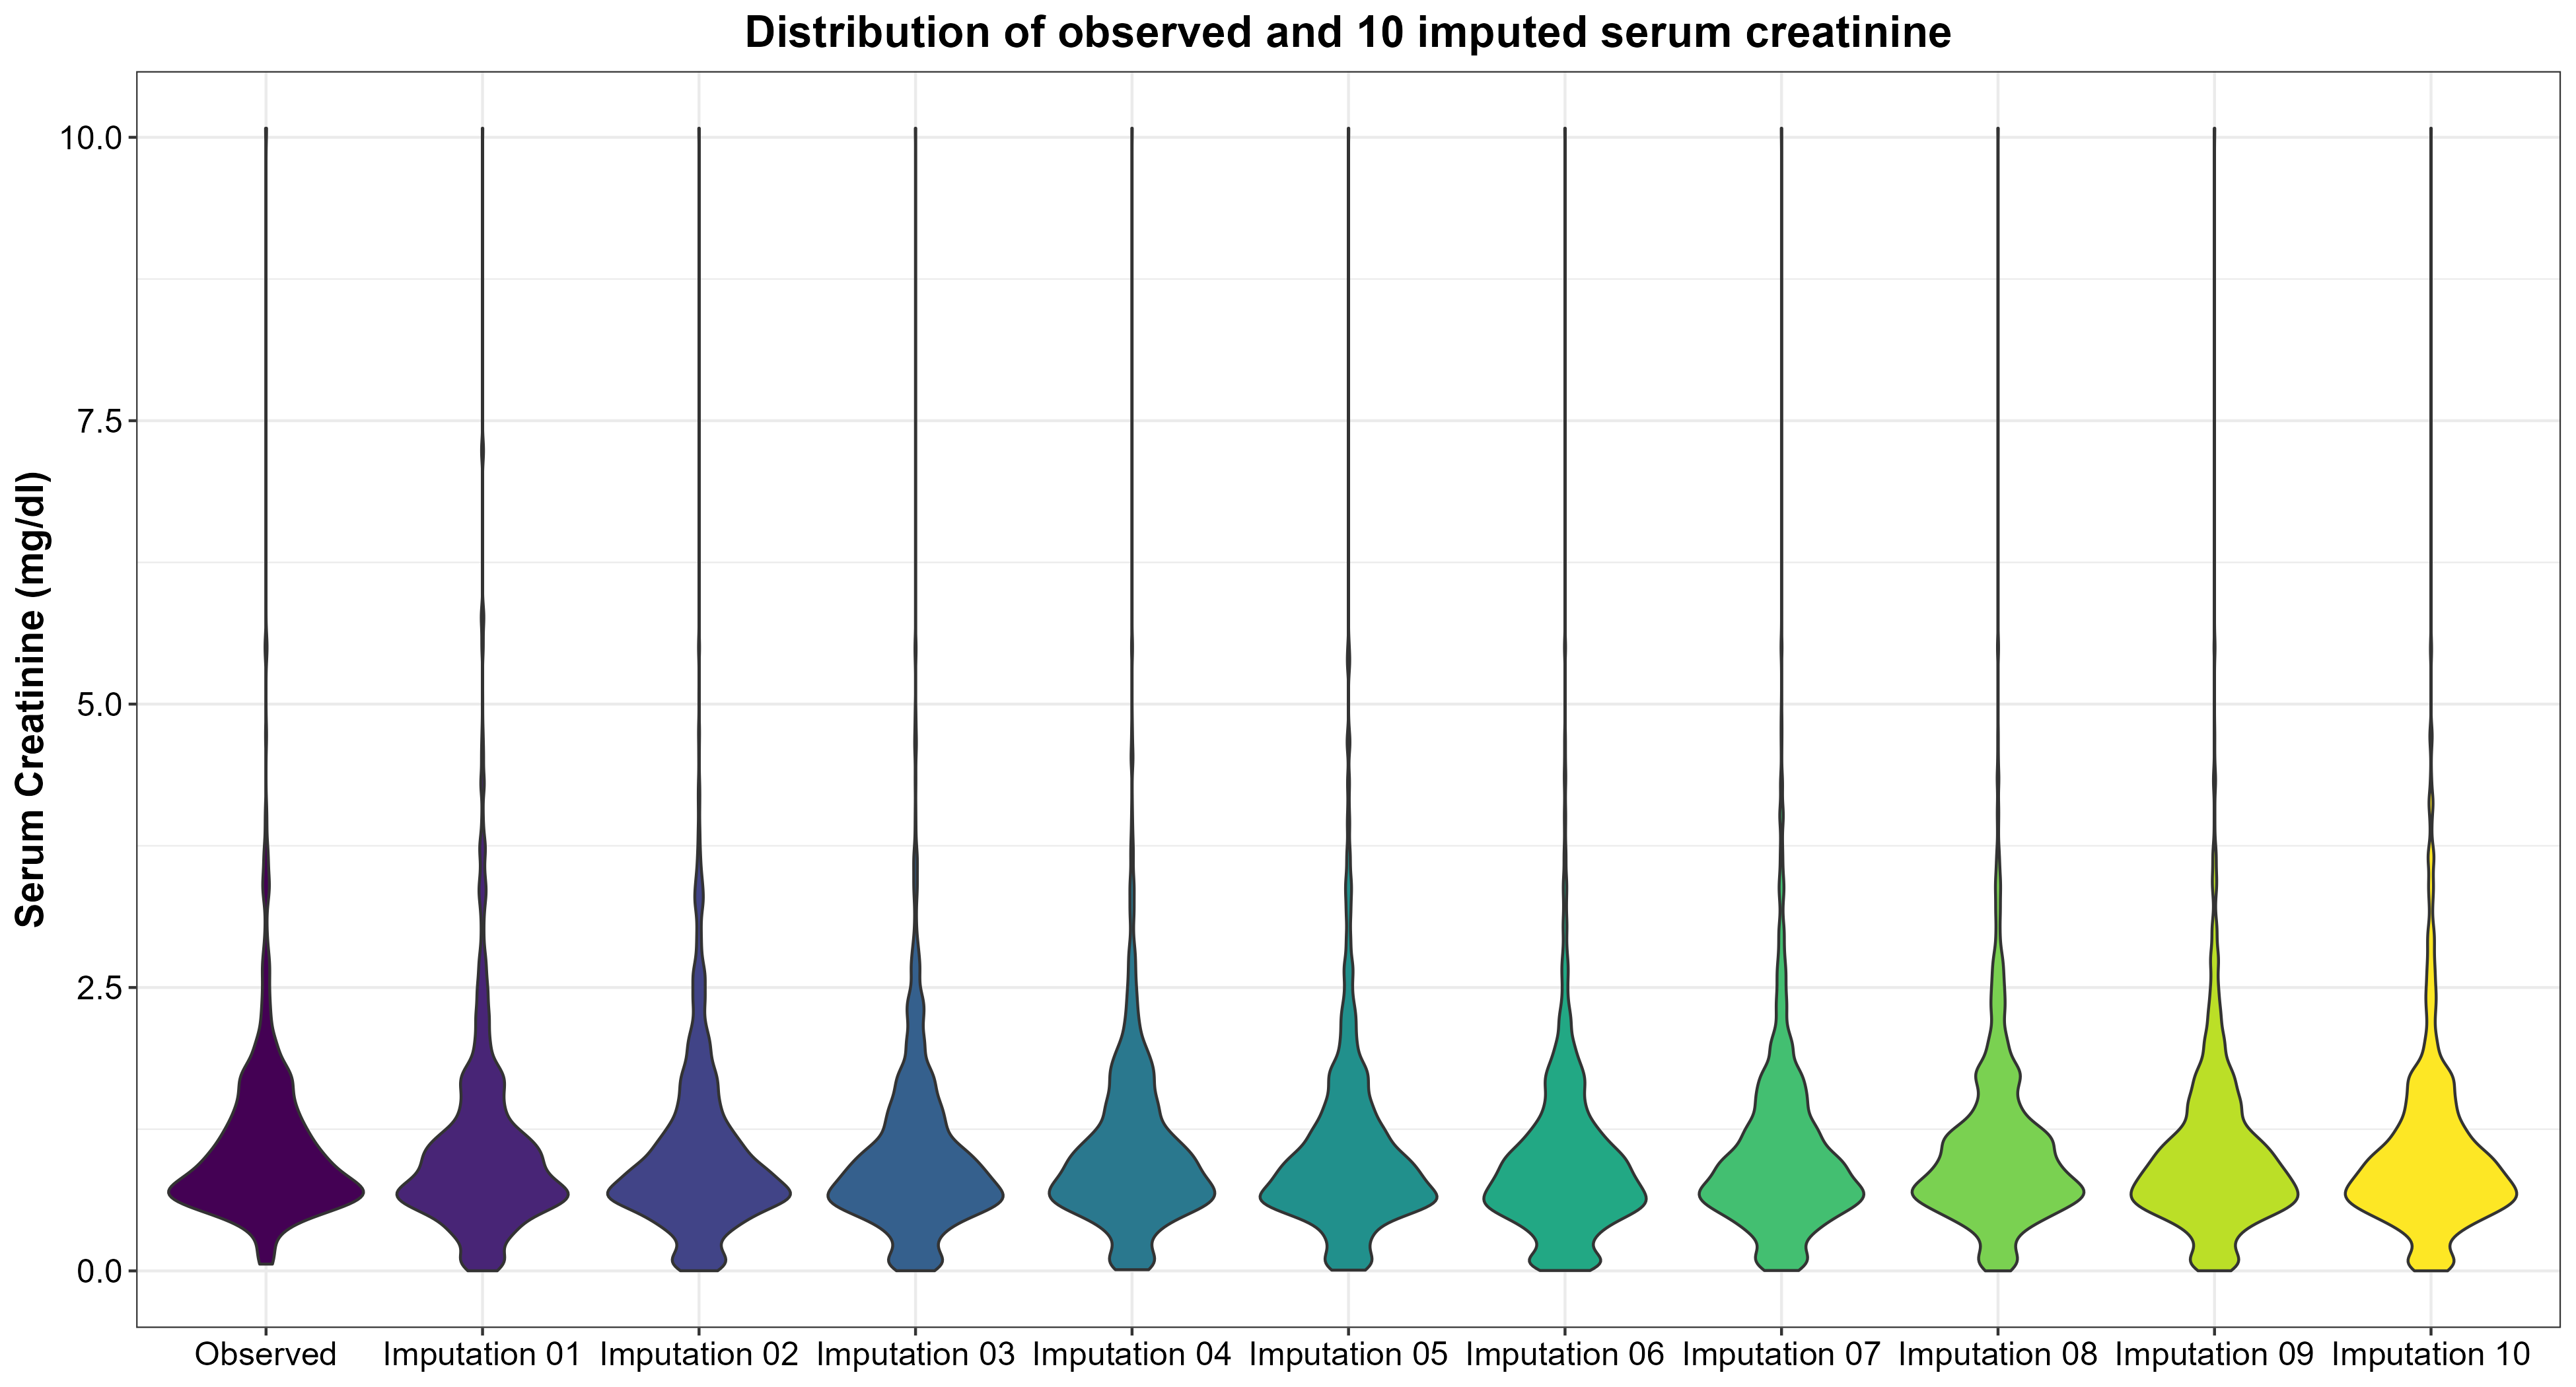
\includegraphics[width=7.01in,height=4.96in]{../../checklist-ijaa/Artwork/figures+captions/supp/figs1-obs_vs_imp_violin.png}

\caption{Violin plot showing the distribution of 10 imputed sets of serum creatinine values and the observed one.}

\end{suppfig}
\end{landscape}

\begin{landscape}

\begin{suppfig}

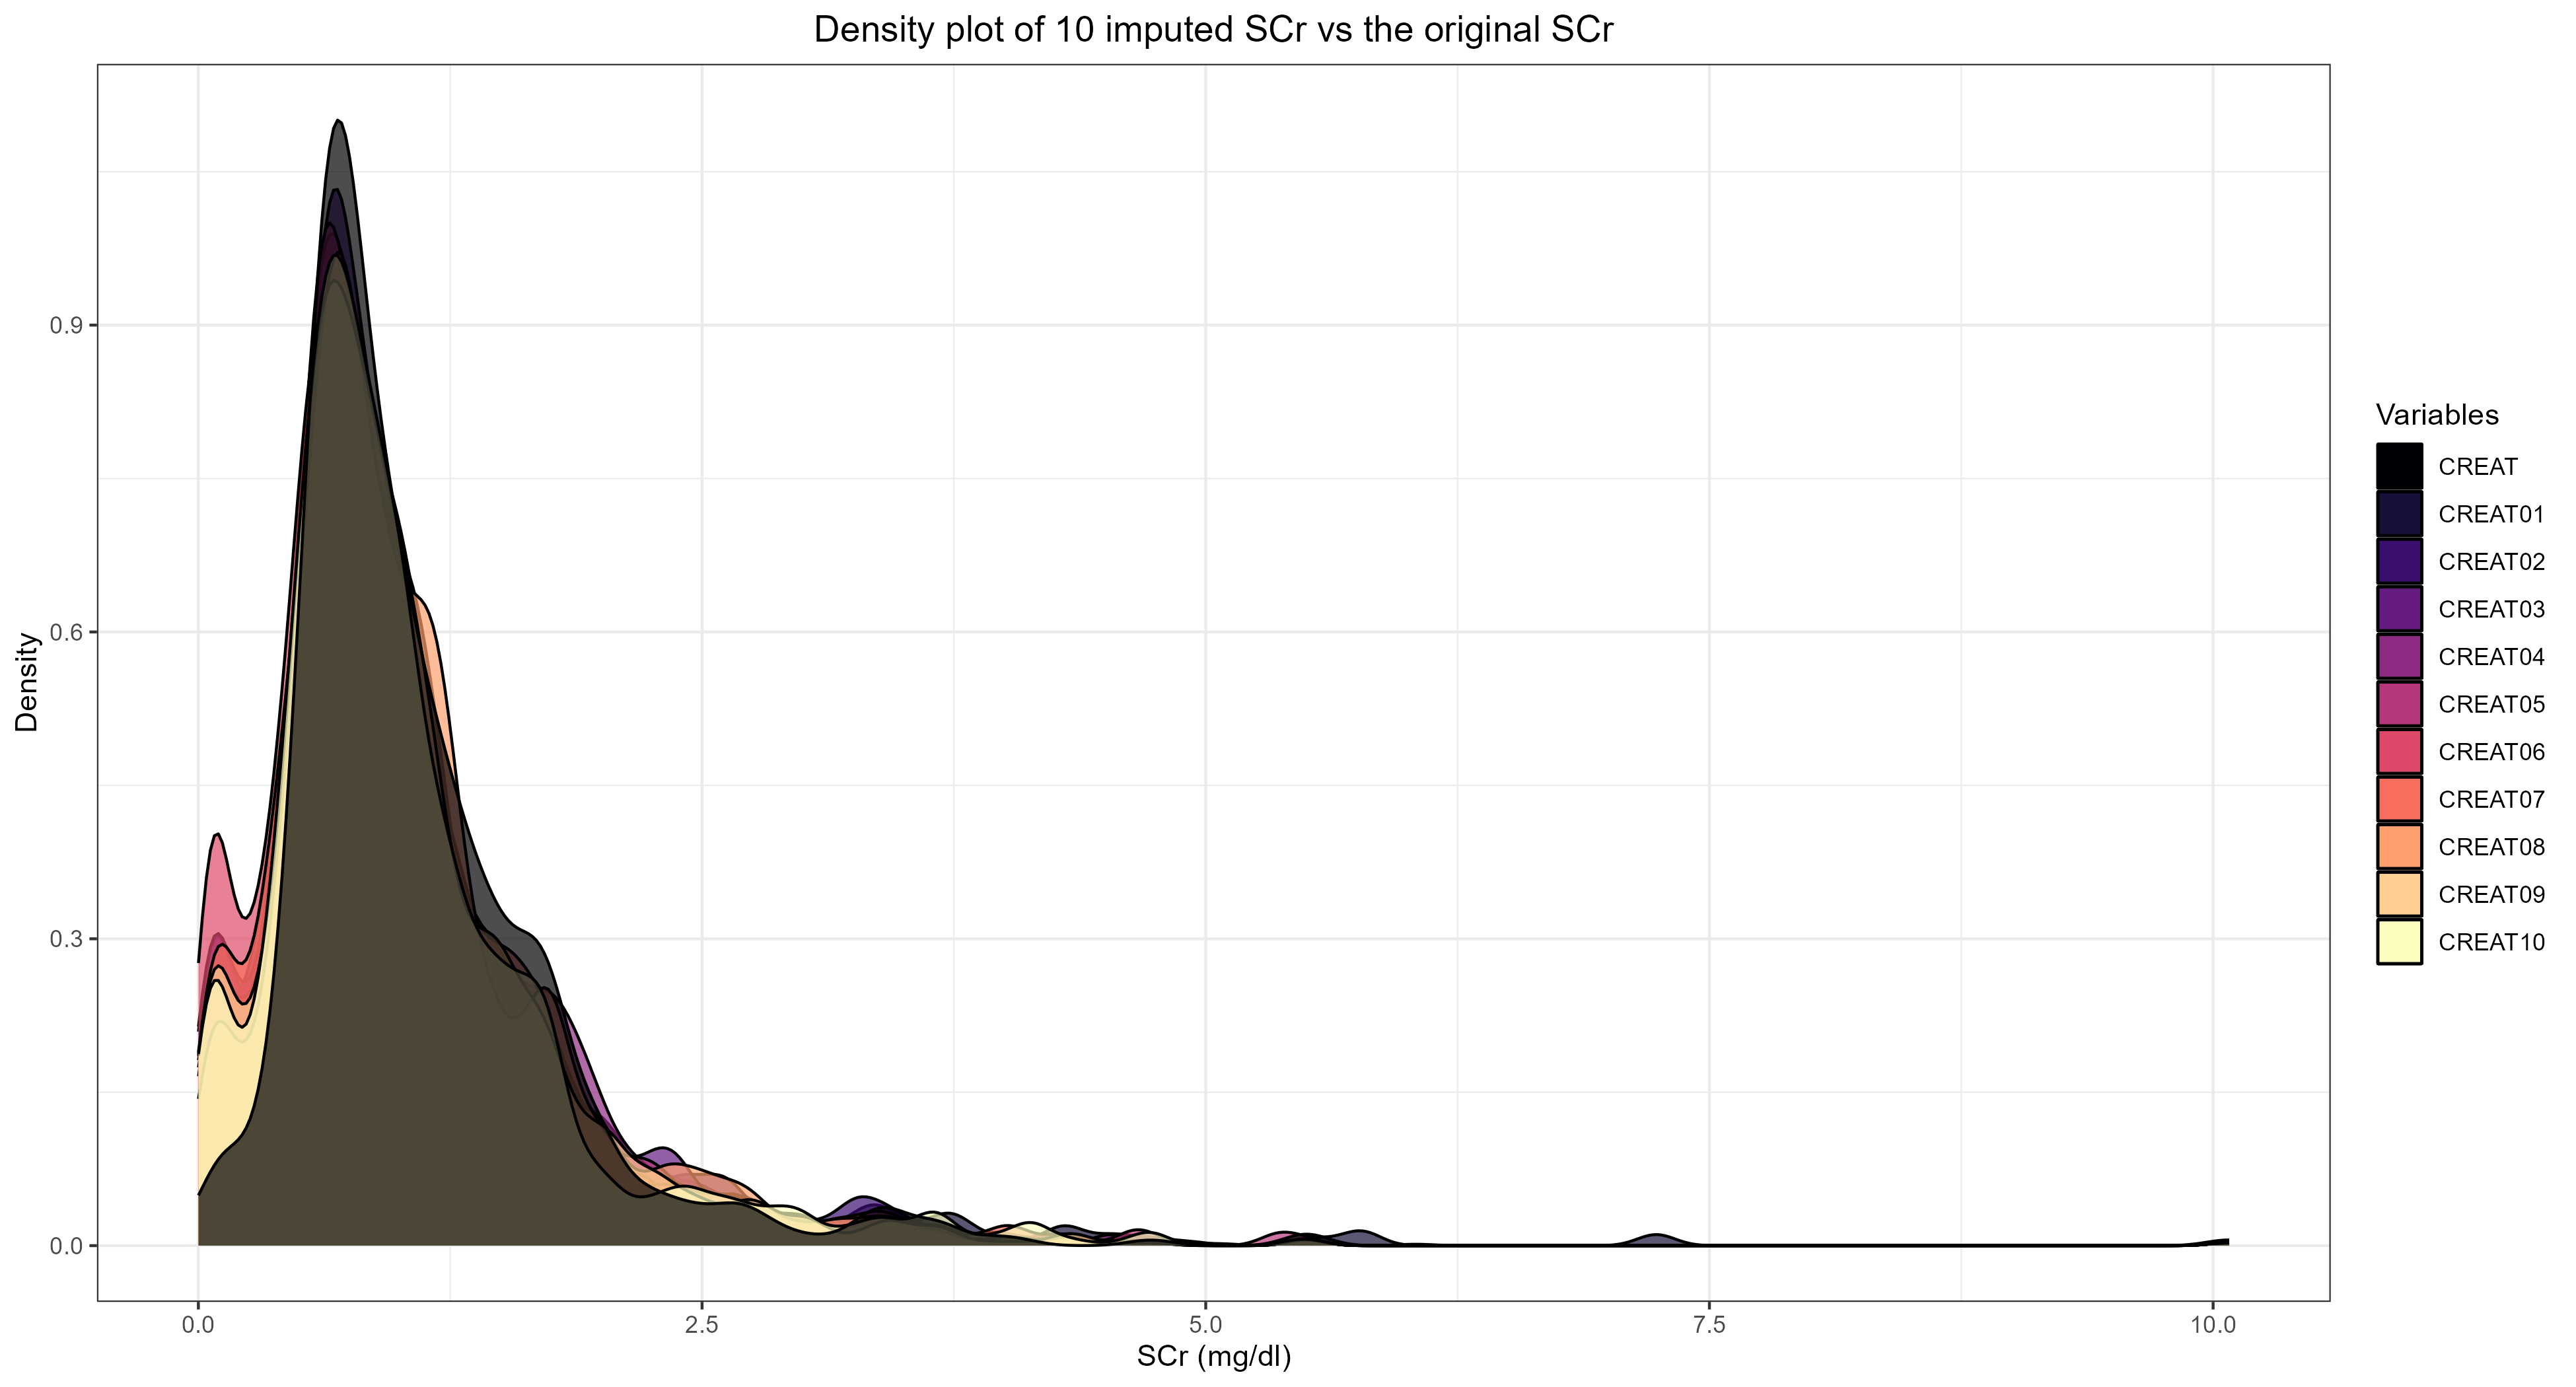
\includegraphics[width=8.18in,height=5.79in]{../../checklist-ijaa/Artwork/figures+captions/supp/figs2-density_plot.png}

\caption{\label{figs-fluco-mi-scr-density}Density plot showing the
distribution of 10 imputed sets of serum creatinine values and the
observed one.}

\end{suppfig}%

\end{landscape}




\end{document}
